% Universidade Aberta
% Template TeX para relatório de trabalhos
% 2025
%
%
% Dados para a capa
\newcommand{\Titulo}{Planeamento e Desenvolvimento de Sistemas de Informação}
\newcommand{\SubTitulo}{Trabalho Grupo - Topico 4}
\newcommand{\Ano}{2025}
\newcommand{\Autor}{
    Pedro Morais - 2401849 \\
    Hugo Gonçalves - 2100562 \\
    Pedro Moro - 2001642 \\
    Luis Peixoto - 2402741 \\
}
%
%
\documentclass[12pt,a4paper,final]{article}
\usepackage{csquotes}
\usepackage{float}
\usepackage[portuguese]{babel}
\usepackage{polyglossia}
\setdefaultlanguage{portuguese}
\usepackage{graphicx}
\graphicspath{ {./images/} }
\usepackage[a4paper,top=3cm,bottom=3cm,left=3.5cm,right=2cm]{geometry}
\usepackage{booktabs}
\setmainfont{Times New Roman}
\defaultfontfeatures{Ligatures=TeX}
\usepackage[pdfauthor=\Autor,
    pdftitle=\Titulo,
    colorlinks=true,
    linkcolor=black,
    citecolor=black,
    bookmarksopen=true]{hyperref}
\hypersetup{colorlinks, citecolor=black, urlcolor=black}
\usepackage{bookmark}
\usepackage[style=apa, backend=biber, sortcites, url=true, language=portuguese]{biblatex}
\usepackage{fontspec}
\DeclareLanguageMapping{portuguese}{portuguese-apa}
\addbibresource{ref.bib}
\renewcommand{\baselinestretch}{1.5}
\begin{document}
    \title{\Titulo}
    \author{\Autor}
    \date{\Ano}
    \pagenumbering{gobble}
    \begin{titlepage}
        \begin{center}
            \vspace*{4cm}

            \textbf{\large UNIVERSIDADE ABERTA}

            \textbf{\large UNIVERSIDADE DE TRÁS-OS-MONTES E ALTO DOURO}

            \vspace{1cm}

            \begin{minipage}{0.4\textwidth}
                \centering
                
\includegraphics[width=0.8\textwidth]{uab}
            \end{minipage}
            \begin{minipage}{0.4\textwidth}
                \centering
                
\includegraphics[width=0.8\textwidth]{utad}
            \end{minipage}

            \vspace{1.5cm}

            \textbf{\large \Titulo}

            \textbf{\large \SubTitulo}

            \vspace{1.5cm}

            \textbf{\large \Autor}

            \vspace{2cm}

            \textbf{\large Mestrado em Engenharia Informática e Tecnologia Web}
            \vfill
            \textbf{\Ano}
        \end{center}
    \end{titlepage}
    \renewcommand{\contentsname}{Índice}
    \cleardoublepage
    \pagenumbering{roman}
    \tableofcontents
    \newpage
    \listoffigures
    \newpage
    \cleardoublepage
    \pagenumbering{arabic}

    \section*{Introdução}\label{sec:introducao}
    \addcontentsline{toc}{section}{Introdução}
    No âmbito da unidade curricular, foi‑nos colocado o desafio de delinear a arquitectura de negócio de um projecto que pretende transformar Lisboa numa «cidade inteligente».
    Nesta segunda fase, procedeu‑se ao levantamento das entidades de informação da Direcção Municipal de Higiene
    Urbana (DMHU), e identificou‑se os diversos órgãos, intervenientes e demais entidades relevantes.

A entrega segue o proposto no enunciado, respondendo às duas questões:
    \begin{itemize}
        \item Q7 - Summary of DMHU information entities, including its classification according to Immon.
        \item Q8 - Detailed domain model for the information entities
    \end{itemize}



    \section*{Q7 - Sumário das Entidades de Informação da DMHU}
    \addcontentsline{toc}{section}{Q7 - Sumário das Entidades de Informação DMHU}

    Seguidamente, apresentamos a arquitetura de informação proposta para a DHMU. Verifica-se que a Direção dispõe
    de várias aplicações para acesso aos sistemas legados, estando em curso propostas de alteração que foram consideradas nesta arquitetura.

    Constatamos um elevado número de aplicações destinadas a diversos fins dentro da DHMU (projetos, relatórios de auditoria, entre outros) que podem sofrer alterações significativas ao longo do tempo, embora recorram aos dados já disponíveis.

    Isto, aliado à recente tendência de disseminação de soluções de Business Intelligence e Advanced Analytics,
    leva-nos a propor a criação de uma camada de informação na DHMU, a qual permitirá que todas as unidades criem
    aplicações analíticas de forma autónoma, sem impactar os dados transacionais.

    A Tabela~\ref{tab:inmon} sintetiza as principais entidades identificadas nas
    camadas Transacional e de \textit{Business Intelligence} (BI), atribuindo-lhes a
    classificação proposta por Inmon para um armazém de dados—\emph{current
    detail}, \emph{lightly summarized} ou \emph{historical detail}—consoante a sua
    granularidade e horizonte temporal.


    \begin{table}[H]
        \centering
        \caption{Classificação Inmon das entidades de informação da DMHU}
        \label{tab:inmon}
        \begin{tabular}{@{}|c|c|c|@{}}
            \toprule
            \textbf{Entidade} & \textbf{Identificador (PK)} & \textbf{Classificacao Inmon}\\\midrule
            Equipamentos\_Execucao          & \texttt{ExecucaoID}         & Current detail\\
            Cadastro\_Circuitos             & \texttt{CircuitoID}         & Current detail\\
            Execucao\_Diária                & \texttt{ExecucaoID}         & Current detail\\
            Escala\_Circuitos               & \texttt{EscalaID}           & Current detail\\
            Cadastro\_PRS                   & \texttt{PRSID}             & Current detail\\
            Equipamentos                    & \texttt{EquipamentoID}      & Current detail\\
            Solicitacoes\_Ocorrencias       & \texttt{OcorrenciaID}       & Current detail\\
            Pessoas\_Escala\_Circuitos      & \texttt{PessoaEscalaID}     & Current detail\\
            RH\_Fardamento\_EPI             & \texttt{EPIID}              & Current detail\\
            Manutencao                      & \texttt{ManutencaoID}       & Current detail\\
            Interacoes                      & \texttt{InteracaoID}        & Current detail\\
            Cadastro\_Colaboradores         & \texttt{ColaboradorID}      & Historical detail\\
            Acidentes\_Colaboradores        & \texttt{AcidenteID}         & Historical detail\\
            RH\_SIADAP                       & \texttt{AvaliacaoID}        & Historical detail\\
            RH\_Ocorrencias                 & \texttt{RH\_OcorrenciaID}   & Historical detail\\
            RH\_Formacao\_Colaborador       & \texttt{FormacaoColabID}    & Historical detail\\
            RH\_Acidentes                   & \texttt{AcidenteID}          & Historical detail\\
            RH\_Formacao                   & \texttt{FormacaoID}        & Historical detail\\
            Orcamento                       & \texttt{OrcamentoID}    & Historical detail\\
            \midrule
            \multicolumn{3}{p{12cm}}{\textit{Nota:} as réplicas diárias destas entidades na
            camada BI são classificadas como \emph{lightly summarized}, correspondendo a
            snapshots temporais para análise e \textit{report}.}\\
            \bottomrule
        \end{tabular}
    \end{table}

    \newpage

    A Figura~\ref{fig:info-structure} apresenta uma visualização das entidades transacionais, neste caso apenas os
    dados.

    \begin{figure}[H]
        \centering
        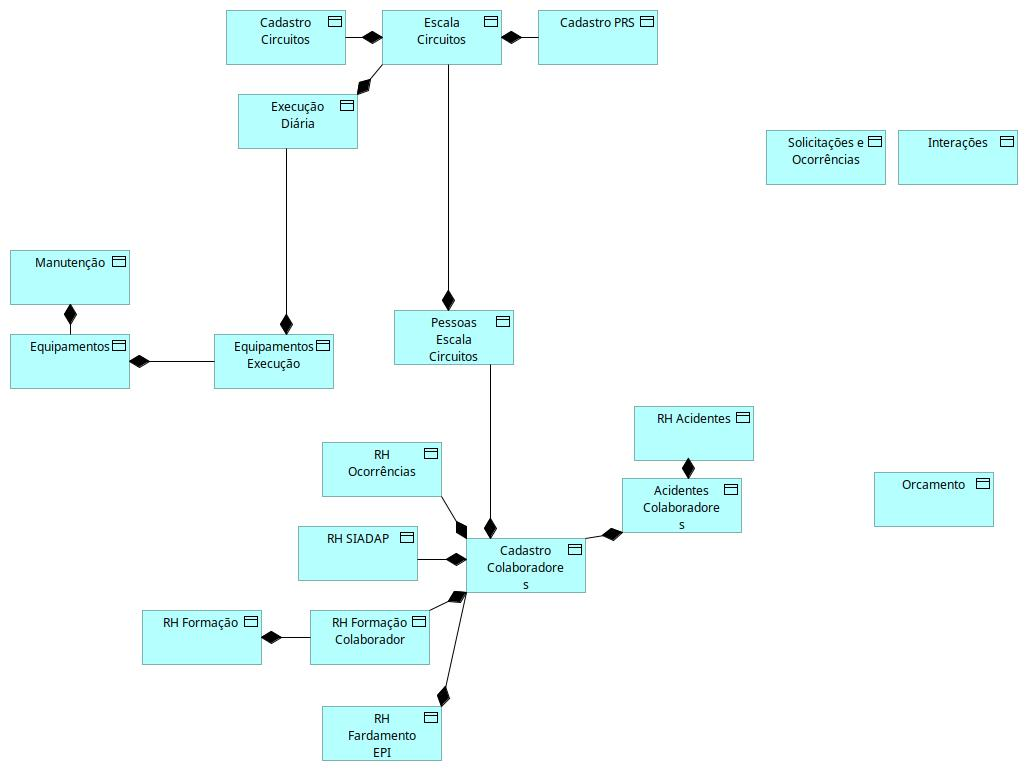
\includegraphics[width=\textwidth]{Q7 Information Architecture - Transacional Apenas Dados}
        \caption{Information Architecture - Visão Transacional Apenas Dados}
        \label{fig:info-structure}
    \end{figure}

    \newpage
    \section*{Q8 - Modelo de Domínio Detalhado}
    \addcontentsline{toc}{section}{Q8 - Modelo de Domínio Detalhado}

    \subsection*{Information Structure - Class Diagram UML}\label{subsec:class-diagram-uml}
    A Figura~\ref{fig:uml-interfaces} apresenta uma visualização das entidades transacionais, uma visão das interfaces.

    \begin{figure}[H]
        \centering
        \includegraphics[width=\textwidth]{Q8 - Information Architecture - Transacional - Visão Interfaces}
        \caption{Information Architecture - Transacional - Visão Interfaces}
        \label{fig:uml-interfaces}
    \end{figure}

    Complementarmente, a Figura~\ref{fig:archi-full} e a Figura~\ref{fig:archi-info} evidência
    como os objetos de dados são replicados e disponibilizados na camada BI,
    estabelecendo a ponte entre dados operacionais e informacionais.

    \begin{figure}[H]
        \centering
        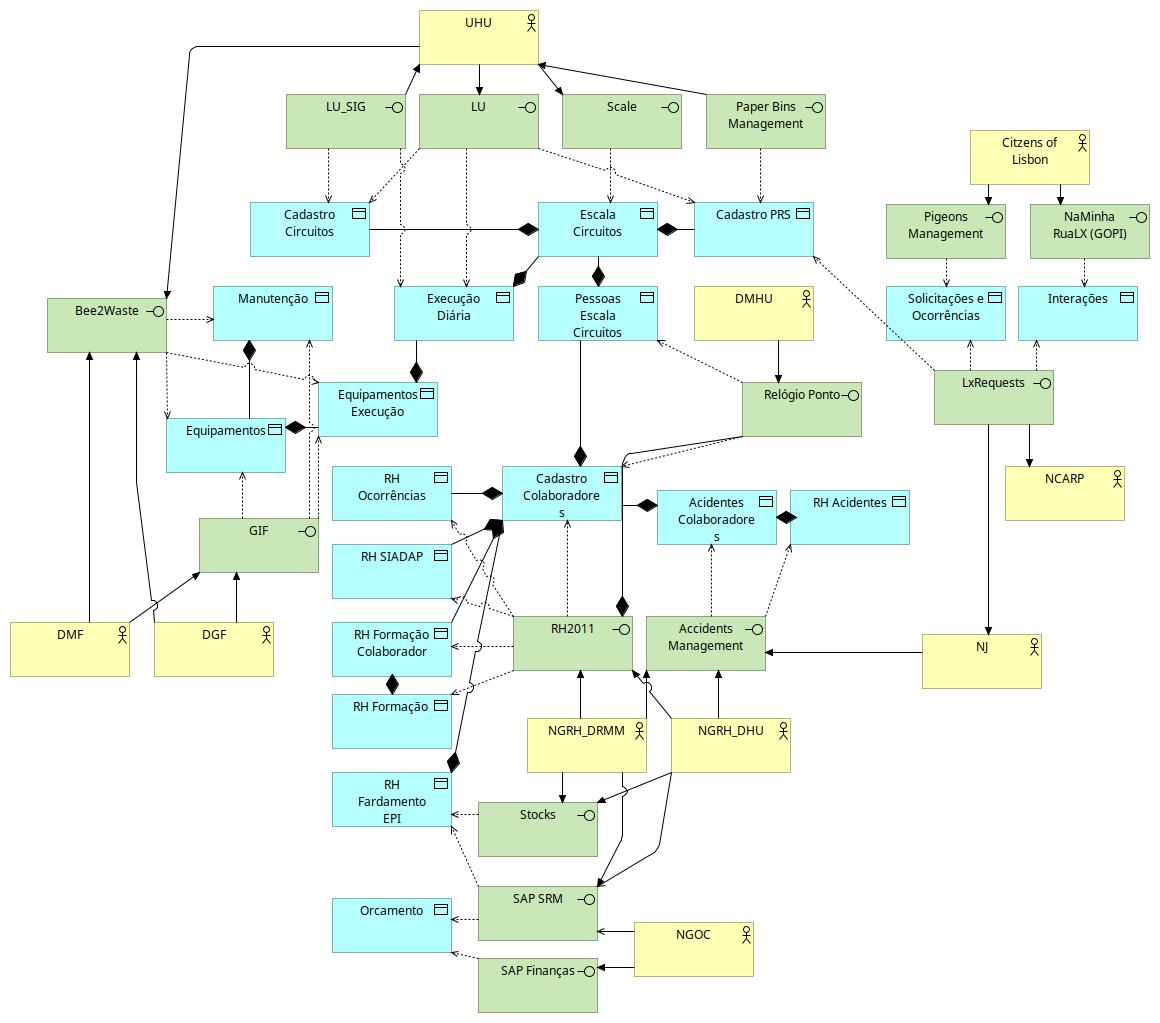
\includegraphics[width=\textwidth]{Q8 - Information Architecture - Transacional}
        \caption{Information Architecture - Visão Transacional}
        \label{fig:archi-full}
    \end{figure}

    \begin{figure}[H]
        \centering
        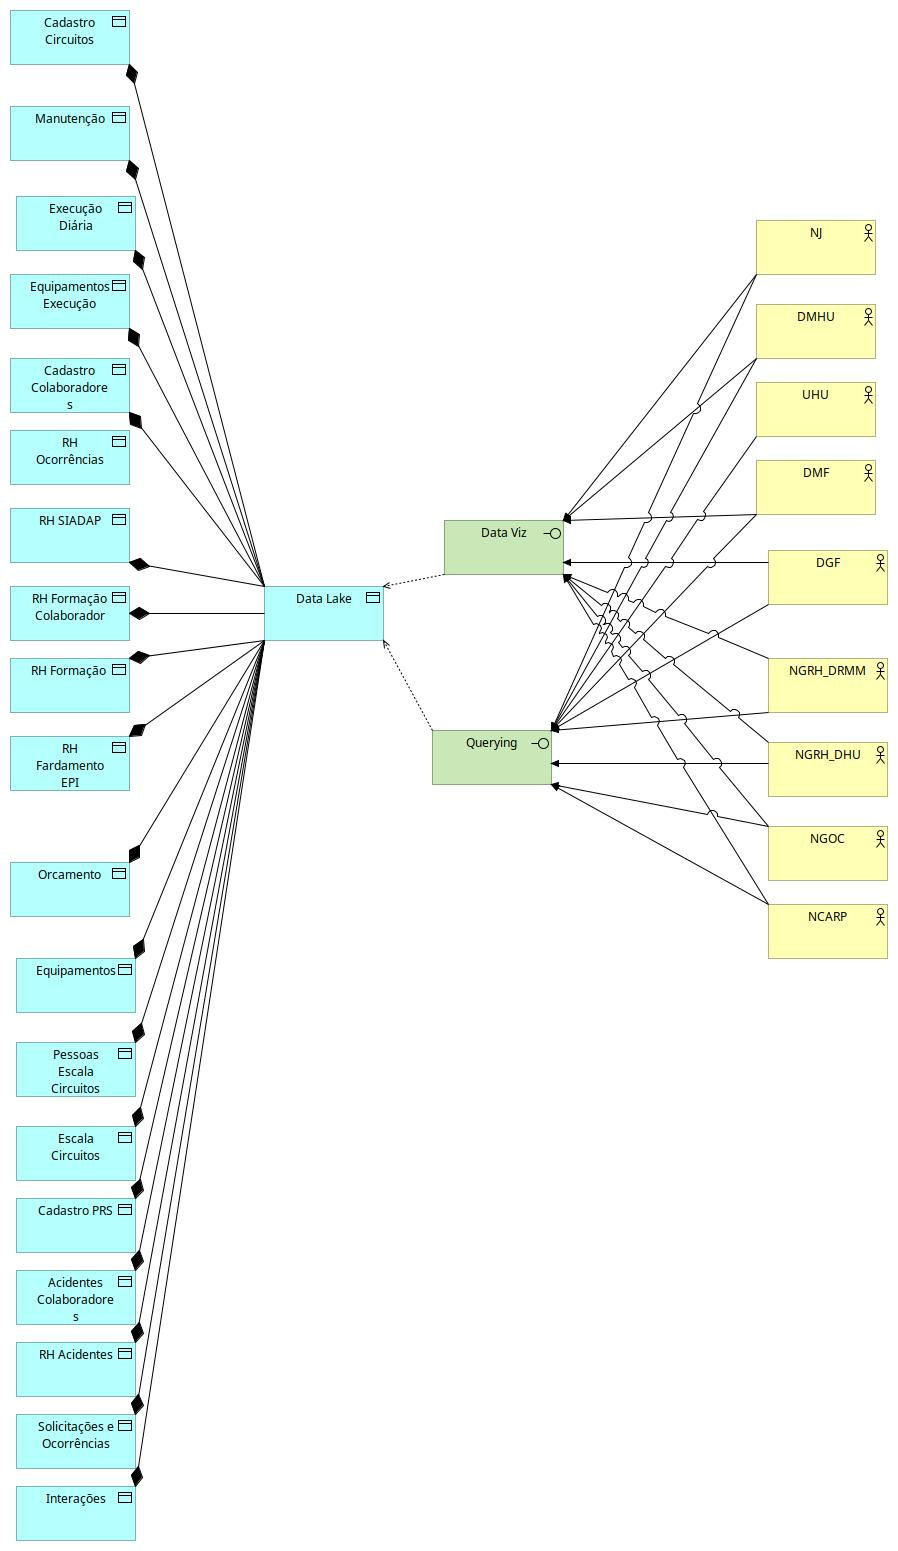
\includegraphics[width=0.8\textwidth]{Q8 - Information Architecture - Informational}
        \caption{Information Architecture - Visão Informational}
        \label{fig:archi-info}
    \end{figure}

    Estas representações asseguram uma visão consistente
    (\emph{traceability}) entre o modelo de domínio e a arquitetura de dados,
    facilitando a evolução futura da solução.

    \subsection*{Detalhes dos Atores}\label{subsec:information-atores}

    Esta seção contém uma definição de cada um dos atores mostrados nos modelos deste relatório, para fins de compreensão serão separados em Atores de negócios (Entidades que fazem uso da arquitetura informacional, sejam da própria DHMU ou externas a ela), Interfaces tecnológicas (Sistemas e aplicações usados pelos atores) e Objetos Informacionais (Representações dos domínios de dados)
\\
    \\
\textbf{Atores de Negócio:}

    \textbf{UHU:} Unidade de Higiene Urbana, com todas as suas divisões geográficas

    \textbf{DMF:} Divisão de Manutenção da Frota

    \textbf{DGF:} Divisão de Gestão da Frota

    \textbf{NGRH:} Núcleos de Gestão de Recursos Humanos, separados por Departamentos

    \textbf{Citzens of Lisbon:} Munícipes de Lisboa de forma geral

    \textbf{NJ:} Núcleo Jurídico

    \textbf{NCARP:} Núcleo de Comunicação, Atendimento e Relações Públicas

    \textbf{DHMU:} Colaboradores da DHMU de uma forma geral, sem distinção da respetiva área

    \textbf{NGOC:} Núcleo de Gestão do Orçamento e Contabilidade
\\
    \\
    \textbf{Interfaces Tecnológicas:}

    \textbf{Bee2Waste:} Aplicação para gestão do ciclo de vida dos ativos

    \textbf{GIF:} Aplicação para gestão da frota

    \textbf{LU:} Limpeza Urbana, gerenciamento dos processos de coleta urbana

    \textbf{LU\_SIG:} Limpeza Urbana - Gerenciamento geográfico de circuitos

    \textbf{Scale:} Gerenciamento de escalas de serviço dos colaboradores

    \textbf{Paper Bins Management:} Sistema para gerenciamento especifico dos pontos de coleta de papéis

    \textbf{Pigeons Management:} Inclui o sistema Lx Requests, ambos se referem ao relato de pontos de concentração
    de Pombos

    \textbf{NaMinha RuaLX (GOPI):} Sistema principal de interação do Munícipe com a DMHU

    \textbf{LX Requests:} Aplicação interna, permite gerenciamento dos pedidos, reclamações e pedidos registrados pelos munícipes

    \textbf{Accidents Management:} Novo Sistema de gerenciamento de acidentes no ambiente de trabalho. Desenvolvido em Oracle APEX – Substituirá o sistema SST

    \textbf{RH2011:} Sistema para gestão dos assuntos de Recursos Humanos

    \textbf{Relógio Ponto:} Aplicação de relógio ponto. É gerida pelos núcleos de RH, mas todos os funcionários da DMHU elegíveis ao controle de ponto a acessam para registrar seus horários de entrada e saída

    \textbf{Stocks:} Sistema de gerenciamento de requisições de material e uniformes

    \textbf{SAP:} apresenta duas Interfaces, a SRM (Supplier Relationship Management) que gerencia pedidos de insumos ao armazém central da Câmara de Lisboa. E a Finanças, aonde ocorre a gestão financeira da DMHU.
\\
    \\
    \textbf{Objetos Informacionais:}

    \textbf{Cadastro Circuitos:} Cadastro dos circuitos operados pela DMHU, sejam eles de recolha ou não

    \textbf{Cadastro PRS:} Cadastro dos pontos de recolha seletiva que compõe um circuito

    \textbf{Escala Circuitos:} Tabela de Relacionamentos, Cada Circuito pode ter múltiplos PRS e Execuções diárias

    \textbf{Execução Diária:} contém informações sobre a execução diária e horários de visita aos PRS.

    \textbf{Equipamentos Execução:} Contém os equipamentos usados em cada execução

    \textbf{Equipamentos:} Cadastro dos equipamentos de posse da DMHU

    \textbf{Manutenção:} Agenda de manutenção dos equipamentos

    \textbf{Cadastro Colaboradores:} Cadastro de colaboradores da DMHU, serve como Golden Source das informações únicas de um colaborador

    \textbf{Pessoas Escala Circuitos:} Tabela Relacionamentos, Cada Execução pode ter múltiplos colaboradores e vice versa

    \textbf{RH Acidentes:} Registro dos acidentes de trabalho ocorridos

    \textbf{Acidentes Colaboradores:} Tabela Relacionamentos, Cada Acidente pode ter múltiplos colaboradores e vice versa

    \textbf{RH Ocorrências:} registro de ocorrências de RH, Férias, Promoções, contratações, desligamentos, etc.

    \textbf{RH SIADAP:} Fichas de avaliação de desempenho

    \textbf{RH Formação:} Registro das formações disponíveis

    \textbf{RH Formação Colaborador:} Tabela de relacionamentos, cada formação pode ser frequentada por múltiplos colaboradores e um colaborador pode frequentar múltiplas formações

    \textbf{RH Fardamento EPI:} Registro dos fardamentos e EPI’s à disposição da DMHU e respectiva alocação

    \textbf{Orçamento:} Registro das transações financeiras da DMHU

    \textbf{Solicitações e Ocorrências:} Registro de solicitações e ocorrências feitas pelos munícipes

    \textbf{Interações:} Registro de demais interações do Munícipe com a DMHU.

    \newpage
    \nocite{*}
    \printbibliography
\end{document}